\documentclass[11pt,a4paper,twoside]{article}

% ----------------------------------------------------------------------
% Define external packages, language, margins, fonts and new commands
% ----------------------------------------------------------------------
%\input{preamble} 
\usepackage[utf8]{inputenc}   % <<<<< Linux
\usepackage[english]{babel} % <<<<< English
\usepackage{notoccite}
\usepackage[skip=0.5\baselineskip]{caption}
\hyphenation{GTKWave}
\usepackage{listings}
\usepackage[all]{nowidow}
\usepackage{amsmath}
\usepackage{multicol}

%blind text
\usepackage{lipsum}

\usepackage{graphicx}
\graphicspath{{./}{../../figlib/}{../mat/}{../sim/}}
\def\FontLn{% 16 pt normal
  \usefont{T1}{phv}{m}{n}\fontsize{16pt}{16pt}\selectfont}
\def\FontLb{% 16 pt bold
  \usefont{T1}{phv}{b}{n}\fontsize{16pt}{16pt}\selectfont}
\def\FontMn{% 14 pt normal
  \usefont{T1}{phv}{m}{n}\fontsize{14pt}{14pt}\selectfont}
\def\FontMb{% 14 pt bold
  \usefont{T1}{phv}{b}{n}\fontsize{14pt}{14pt}\selectfont}
\def\FontSn{% 12 pt normal
  \usefont{T1}{phv}{m}{n}\fontsize{12pt}{12pt}\selectfont}

% Use Arial font as default
%
\renewcommand{\rmdefault}{phv}
\renewcommand{\sfdefault}{phv}
\usepackage{geometry}	
\geometry{verbose,tmargin=2.5cm,bmargin=2.5cm,lmargin=2.5cm,rmargin=2.5cm}

%\usepackage{setspace}
%\renewcommand{\baselinestretch}{1.5}

\usepackage[pdftex]{hyperref} % enhance documents that are to be
                              % output as HTML and PDF
\hypersetup{colorlinks,       % color text of links and anchors,
                              % eliminates borders around links
%            linkcolor=red,    % color for normal internal links
            linkcolor=black,  % color for normal internal links
            anchorcolor=black,% color for anchor text
%            citecolor=green,  % color for bibliographical citations
            citecolor=black,  % color for bibliographical citations
%            filecolor=magenta,% color for URLs which open local files
            filecolor=black,  % color for URLs which open local files
%            menucolor=red,    % color for Acrobat menu items
            menucolor=black,  % color for Acrobat menu items
%            pagecolor=red,    % color for links to other pages
            pagecolor=black,  % color for links to other pages
%            urlcolor=cyan,    % color for linked URLs
            urlcolor=black,   % color for linked URLs
	          bookmarks=true,         % create PDF bookmarks
	          bookmarksopen=false,    % don't expand bookmarks
	          bookmarksnumbered=true, % number bookmarks
	          pdftitle={report},
            pdfauthor={Grupo 36 TCFE MEFT 21},
%            pdfsubject={Thesis Title},
%            pdfkeywords={Thesis Keywords},
            pdfstartview=FitV,
            pdfdisplaydoctitle=true}

\usepackage[numbers,sort&compress]{natbib} % <<<<< References in numbered list [1],[2],...
\usepackage{subcaption} 
\usepackage{mdframed}

%%%%%%%%%%%%%%%%%%%%%%%%%%%%%%%%%%%%%%%%%%%%%%%%%%%%%%%%%%%%%%%%%%%%%%%%
%     Begin Document                                                   %
%%%%%%%%%%%%%%%%%%%%%%%%%%%%%%%%%%%%%%%%%%%%%%%%%%%%%%%%%%%%%%%%%%%%%%%%


\begin{document}

% Set plain page style (no headers, footer with centered page number)
\pagestyle{plain}

% Set roman numbering (i,ii,...) before the start of chapters
%\pagenumbering{roman}

% ----------------------------------------------------------------------
%  Cover page
% ----------------------------------------------------------------------
%%%%%%%%%%%%%%%%%%%%%%%%%%%%%%%%%%%%%%%%%%%%%%%%%%%%%%%%%%%%%%%%%%%%%%%%
%                                                                      %
%     File: Thesis_FrontCover.tex                                      %
%     Tex Master: Thesis.tex                                           %
%                                                                      %
%     Author: Andre C. Marta                                           %
%     Last modified :  2 Jul 2015                                      %
%                                                                      %
%%%%%%%%%%%%%%%%%%%%%%%%%%%%%%%%%%%%%%%%%%%%%%%%%%%%%%%%%%%%%%%%%%%%%%%%

\thispagestyle {empty}

% IST Logo - Signature A
% parameters: bb=llx lly urx ury (bounding box), width=h_length, height=v_length, angle=angle, scale=factor, clip=true/false, draft=true/false. 

\includegraphics[bb=9.5cm 11cm 0cm 0cm,scale=0.29]{IST_A_CMYK_POS}

\begin{center}
%
% Figure (Image or plot)
\vspace{1.0cm}
% height = 50 mm
%\includegraphics[height=50mm]{Figures/Airbus_A350.jpg}

% Title, author and degree
\vspace{1cm}
{\FontLb Lab 3: ACDC converter} \\ % <<<<< EDIT TITLE
\vspace{1cm}
{\FontSn Master’s programme in Engineering Physics (MEFT), Instituto Superior Técnico, University of Lisbon} \\ % <<<<< EDIT COURSE
\vspace{0.6cm}
{\FontSn Circuit Theory and Electronics Fundamentals} \\
\vspace{0.6cm}
{\FontSn Ana Almeida 96505 \\ Francisco Simões 96526 \\ Juna Santos 96549} \\
\vspace{1cm}
{\FontSn May 8, 2021} \\ % <<<<< EDIT DATE (corresponds to date of oral examination)
%
\end{center}



% ----------------------------------------------------------------------
% Dedication page (optional)
% ----------------------------------------------------------------------
%\input{dedication} 
%\cleardoublepage

% ----------------------------------------------------------------------
%  Acknowledgments (optional)
% ----------------------------------------------------------------------
%\input{acknowledgements}
%\cleardoublepage

% ----------------------------------------------------------------------
%  Abstract (both in English and Portuguese)
% ----------------------------------------------------------------------
%\input{resumo} 
%\cleardoublepage

%\input{abstract} 

% ----------------------------------------------------------------------
%  Table of contents, list of tables, list of figures and nomenclature
% ----------------------------------------------------------------------

% Table of contents
%
\tableofcontents
\newpage
% List of tables
%\addcontentsline{toc}{section}{\listtablename}
%\listoftables
%\cleardoublepage 

% List of figures
%\addcontentsline{toc}{section}{\listfigurename}
%\listoffigures
%\cleardoublepage 

% Set arabic numbering (1,2,...) after preface
%
%\setcounter{page}{1}
%\pagenumbering{arabic}

% ----------------------------------------------------------------------
%  Body
% ----------------------------------------------------------------------

\section{Introduction}
\label{sec:introduction}

% state the learning objective 
The objective of this laboratory assignment was to simulate and create an acdc converter
that would minimize the cost of the components while decreasing the ripple of output.
We used Octave for a theoretical analysis of the circuit and Ngspice to simulate it.
The values of both analysis are compared at the end of this document.
The units of the cost is MU (monetary unit).
The merit of our circuit is given by the following expression:

\begin{equation}
    M = \frac{1}{cost(ripple(v_0)+average(v_0-12)+10^{-6})}
\end{equation}\par

Where: \par
cost = cost of Resistors + cost of Capacitors + cost of Diodes \par
cost of Resistor = 1 MU per kOhm \par
cost of Capacitor = 1 MU per $\mu$ F \par
cost of Diodes = 0.1 MU per diode \par

\vspace{10mm}
The circuit we built is presented in figure \ref{fig:circuit}.
The transformer in the left side is considerer to be ideal and the ration N1/N2 is approximated to 17.577.
This means that we considered an AC source of 13.0855 V (50Hz) for the rest of the circuit in the right side.

\vspace{-4mm}
\begin{figure}[ht] \centering
    \caption{ACDC converter circuit}
    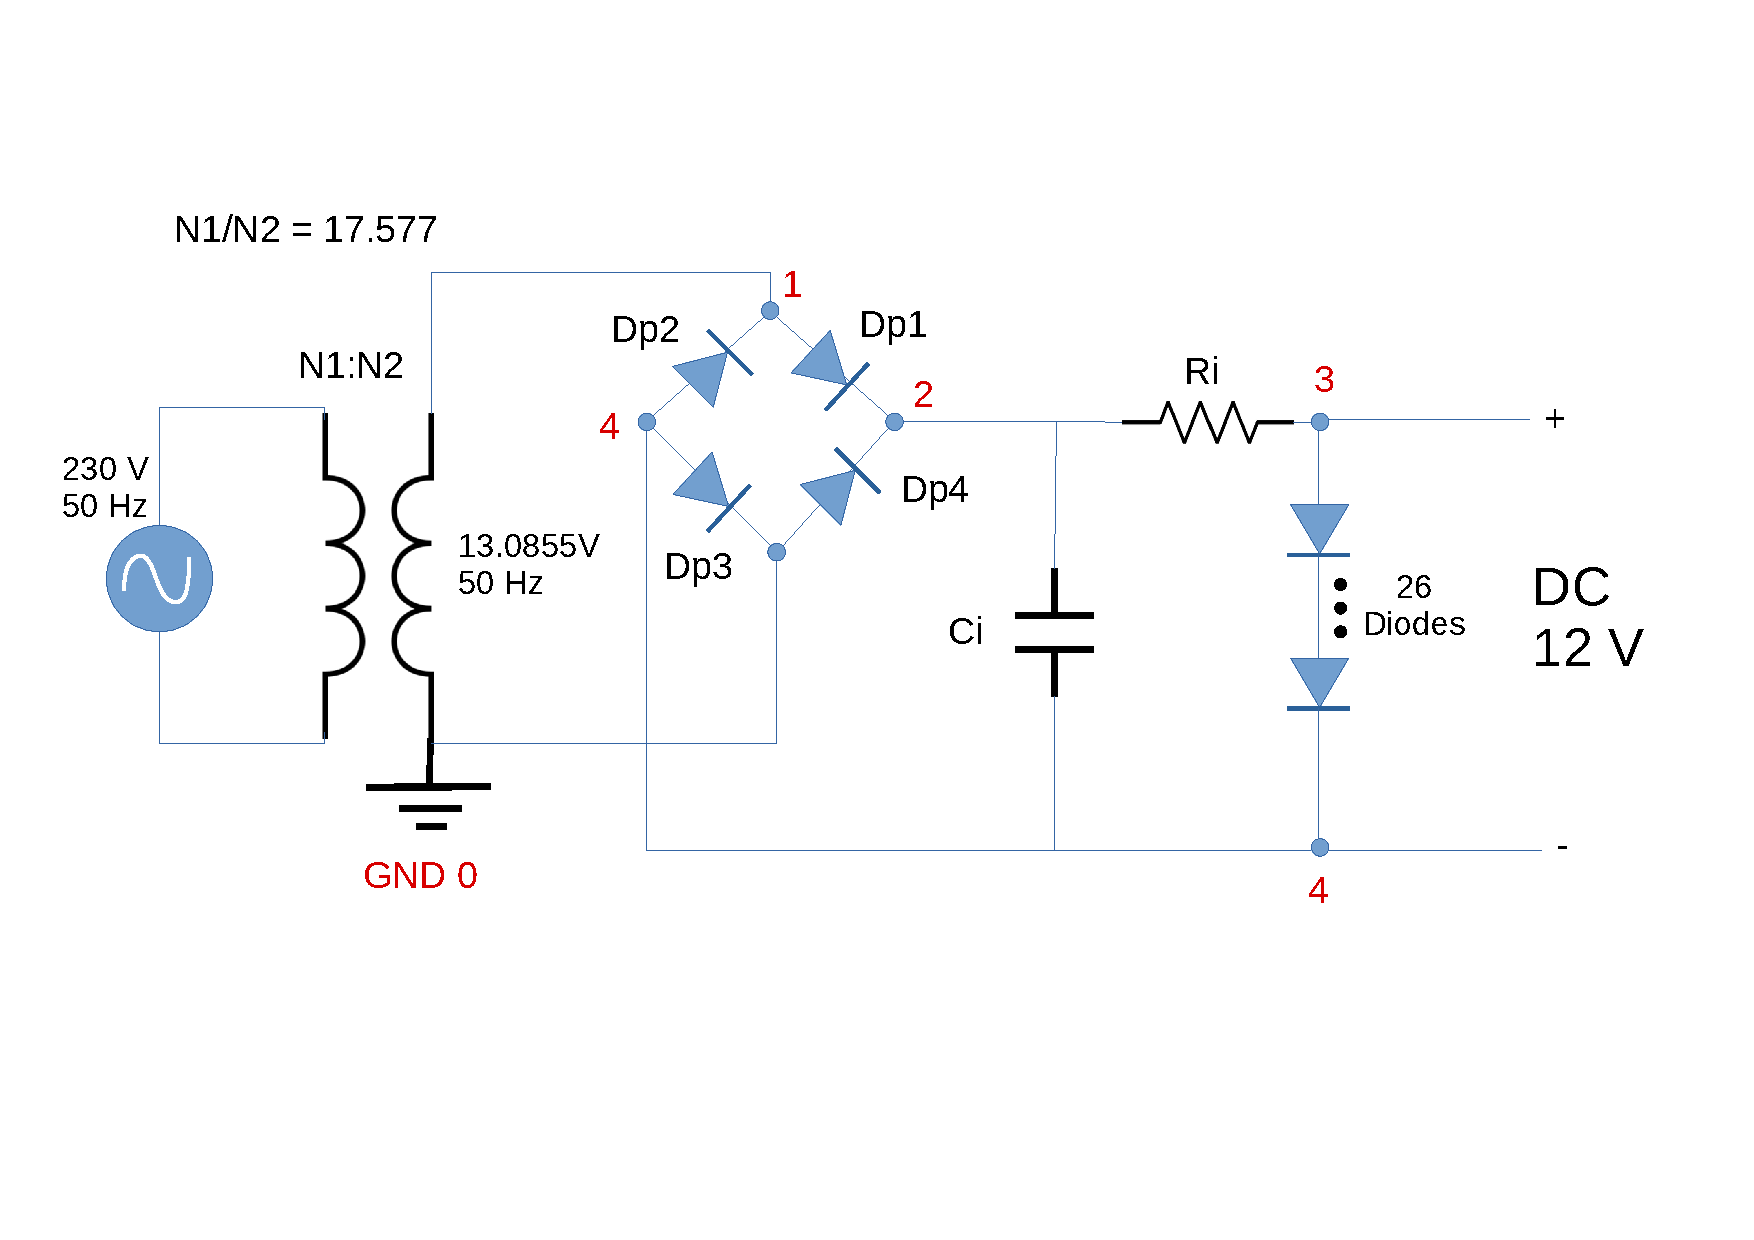
\includegraphics[width=0.8\linewidth]{circuit.pdf}
    \label{fig:circuit}
\end{figure}

\vspace{-6mm}
Components used and respective price are presented in table \ref{tab:material}:
\vspace{5mm}
\begin{table}[ht]
    \centering
    \begin{tabular}{|c|c|c|}
      \hline    
      {\bf Component} & {\bf Quantity or Value} & {\bf Cost} \\ \hline
      Resistor (Ri) & 13.6 kOhm & 13.6 MU \\ \hline
      Capacitor (Ci) & 8 uF & 8.0 MU \\ \hline
      Diodes (Dp1-Dp30) & 30 & 3.0 MU \\ \hline
      Total & - & 24.6 MU \\ \hline
    \end{tabular}
    \vspace{5mm}
    \caption{Electrical Components used and respective cost in MU}
    \label{tab:material}
  \end{table}

\newpage

\section{Theoretical Analysis}
\label{sec:analysis}

In this section, the circuit shown in Figure~\ref{fig:rc} is analysed
theoretically in general by applying Node Analysis. 

Resorting to Ohm's Law, Kirchhoff Current Law (KCL) and Supernode it was possible to get all the information contained in the circuit. 

From KCL we know that the sum of currents converging (diverging) in
a node is null

\[ \sum_{i=1}^{n} I\textsubscript{i} = 0 \]


The Node Analysis was based on Kirchhoff Current Law (KCL) and Ohm Law.
In order to obtain the equations of the nodes who have in between them  a current-controlled voltage source, it isn't possible to write the node equation from KCL
These cases are solved with the help of Supernode analysis. This theoretical concept considers two nodes as just one, in between those nodes it must be placed a voltage source. One of the equations consists in the voltage difference between the nodes being the voltage source value. Then, we consider the nodes as just one node and apply Kirchhoff Current Law since the current that leaves one node is the current that arrives at the other node hence the total current in the new node is null. Now, we are able to apply the KCL to the supernode. 


\subsection{Exercise 1}
To determine all the nodal voltages in $t<0$, with a constant voltage source of value $V_s$, we derived 8 different equations to find the voltages and with these
values then found the branch currents using Ohm's Law and other derived expressions. 
Gi represents 1/Ri and Vi is the voltage in node i and all the equations were defined assuming the divergence of the current in the nodes.

\hspace{-35mm}
\begin{gather}
    \begin{bmatrix}
    1    &   0       & 0     &   0 & 0   & 0 & 0 & 0 \\
    -G1  &  G1+G2+G3 & -G2   &   0 & -G3 & 0 & 0 & 0 \\
    0    &   -G2-Kb  & G2    &   0 & Kb  &0  & 0 & 0 \\   
    0    &   0       & 0     &   1 & 0   & 0 & 0 & 0 \\
    0    &   0       & 0     & -Kd \times G6 & 1 & 0 & Kd\times G6 & -1 \\
    0    &   Kb      & 0     &   0 &  -Kd-G5 & G5 & 0 & 0  \\
    0    &   0       & 0     & -G6 & 0 & 0 & G6+G7 & -G7  \\
    0    &  -G3      & 0     & -G4 & G3+G4+G5 & -G5 & -G7 &  G7 \\
    \end{bmatrix}
    \begin{bmatrix}
    V1     \\
    V2     \\
    V3     \\
    V4     \\
    V5     \\
    V6     \\
    V7     \\
    V8     \\
    \end{bmatrix}
    =
    \begin{bmatrix}
    V_s    \\
    0      \\
    0      \\
    0      \\
    0      \\
    0      \\
    0      \\
    0      \\
    \end{bmatrix}
\end{gather}

%\vspace{-12mm}
%\begin{multicols}{2}
\begin{equation}
I\textsubscript{s} = (V2 - V1) \times G1 
\end{equation}
\begin{equation}
I\textsubscript{b} = (V2 - V5) \times Kb 
\end{equation}
\begin{equation}
I\textsubscript{d} = \frac{V2 - V5}{Kd} 
\end{equation}

Due to the constant value of the voltage provided by $v_s(t)$ in $t<0$, all the voltages determined by this 
system of equations are also constant during this time interval. Since the current through a capacitor is dependent on the 
variation of voltage in its terminals, $i = C\frac{dV}{dt}$, we know that $I_c = 0 A$. The values obtained with Octave are
presented in Tab. \ref{tab:oct1}. 

%\break
\vspace{-20mm}
\begin{table}[h]
    \centering
    \begin{tabular}{|l|r|}
      \hline    
      {\bf Name} & {\bf Value [A or V]} \\ \hline
      \input{../mat/node1.tex}
    \end{tabular}
    \caption{Table with values of current (A) and voltage (V) obtained from mesh and node analysis of the circuit using the tool Octave.}
    \label{tab:oct1}
\end{table}

%\end{multicols}

\newpage
\subsection{Exercise 2}
\label{sec:t2}

The purpose of this exercise is to find the initial conditions of the circuit for a time based analysis.
In order to determine the equivalent resistance, R\textsubscript{eq} and the voltage value $V_x$ as seen from the capacitor terminals the following 
process was executed: Vs was equaled to '0', the capacitor was replaced with a voltage source, V\textsubscript{x} = V6 - V8, where V6 and V8 are the 
voltages obtained in the previous subsection and a new nodal analysis was performed to determine the current Ix that goes through the voltage source.

The nodal matrix is very similar to the previous section matrix, in particular, from node 1 to 5 the equations are equal.

To perform this nodal analysis it is vital to take into account the new voltage source since it will occur a new supernode. 

The nodes 5, 6 and 8 form a supernode and the resulting equations are:

\vspace{-2mm}
\begin{equation}
V5 - V8 = V\textsubscript{d} = Kd \times Id = Kd \times \frac{(V4 - V7)}{R6}
\end{equation}
\vspace{-2mm}
\begin{equation}
V6 - V8 = V\textsubscript{x} 
\end{equation}
\vspace{-2mm}
\begin{equation}
\frac{V5 - V4}{R4} + \frac{V5 - V2}{R3} + \frac{V8 - V7}{R7} + Kb\times(V2 - V5) = 0  
\end{equation}
\vspace{-2mm}
\begin{equation}
Vx = V6 - V8 = 8.4929
\end{equation}

The following matrix system has the information of the equations in all the nodes and its resolution leads us to the voltage value in each node. Table 1 contains the value of voltage in each node.

Gi represents 1/Ri and Vi is the voltage in node i.

\vspace{-5mm}
\begin{gather}
    \begin{bmatrix}
    1       &   0       & 0     &   0 & 0 & 0 & 0 \\
    -G1      &   G1+G2+G3       & -G2     &   0 & -G3 & 0 & 0 & 0  \\
    0       &   -G2-Kb       & G2     &   0 & Kb &0&0 & 0  \\   
    0       &   0       & 0     &   1 & 0 & 0 & 0 \\
    0 & 0 & 0 & -kd\times G6 & 1 & 0 & kd\times G6 & -1 \\
    0       &   0       & 0     & 0 &   0 & 1 & 0 & -1  \\
    0       &   0       & 0     &   -G6 & 0 & 0 & G6+G7 & -G7  \\
    0 & Kb-G3 & 0 & -G4 & G3+G4-Kb & 0 & -G7 &  G7 \\
    \end{bmatrix}
    \begin{bmatrix}
    V1     \\
    V2     \\
    V3     \\
    V4     \\
    V5     \\
    V6     \\
    V7     \\
    V8     \\
    \end{bmatrix}
    =
    \begin{bmatrix}
    0     \\
    0      \\
    0      \\
    0     \\
    0     \\
    V\textsubscript{x}      \\
    0      \\
    0   \\
    \end{bmatrix}
\end{gather}

\vspace{-5mm}
\begin{equation}
I\textsubscript{x} = Kb \times(V2-V5) + G5 \times (V6-V5) = 2.7585 \times 10\textsuperscript{-3} A
\end{equation}
\vspace{-3mm}
\begin{equation}
 R\textsubscript{eq} = \frac{V\textsubscript{x}}{I\textsubscript{x}} = 3078.8  \Omega
\end{equation}
\vspace{-3mm}
\begin{equation}
\tau =  R\textsubscript{eq}\times C = 3.1280\times 10\textsuperscript{-3}
\end{equation}
\vspace{-5mm}
\begin{table}[h]
    \centering
    \begin{tabular}{|l|r|}
      \hline    
      {\bf Name} & {\bf Value [A or V]} \\ \hline
      \input{../mat/node2.tex}
    \end{tabular}
    \caption{Table with values of current (A) and voltage (V) obtained from mesh and node analysis of the circuit using the tool Octave.}
    \label{tab:oct2}
\end{table}



\vspace{-7mm}
\subsection{Exercise 3}

With the values obtained in the previous sections, we are know able to find the not trivial natural solution of node 6.
For it to be a natural solution, the voltage source $v_s(t)$ cannot provide any tension, and so we evaluate 
the circuit assuming $v_s = 0 V$.
Knowing that $V_x$ calculated in section \ref{sec:t2} is now the inicial condition for the voltage value in V6, we have

\vspace{-7mm}
\begin{equation}
    V_{6n} (t) = A e^{st} \Rightarrow V_{6n} (0) = V_x \Leftrightarrow A = V_x \Rightarrow V_{6n} (t) = V_x \times e^{-\frac{t}{\tau}} \Leftrightarrow V_{6n} (t) = 8.4929\times e^{-\frac{t\times 10^3}{3.128}}
\end{equation}

\vspace{-1mm}
Finding the equation through the initial condition we can now plot the graph with the temporal evolution of the voltage 
in this node, according to the natural solution.  

\vspace{-4mm}
\begin{figure}[h] 
    \centering
    \includegraphics[width=0.65\linewidth]{../mat/V6n.jpg}
    \caption{Evolution in time [0;20]ms of the voltage value in node 6, associated with the natural solution}
    \label{fig:v6n}
\end{figure}
    


\newpage
\subsection{Exercise 4}
To determine the forced solution V6\textsubscript{f}(t) for f=1KHz the following process was executed:
A phasor voltage source (Vs = 1) was applyed to the circuit, the capacitor C was replaced with its impedance, $Z_C$, 
and ultimately  the nodal analysis was performed to determine the phasor voltages in all nodes

V6 forced solution must resemble
\begin{equation}
V6\textsubscript{f} = Im\{A\times e^{wt} e^{\phi}\} = A\times sin(w\times t + \phi)
\end{equation}

where, 
\begin{equation}
\omega = 2\times pi\times f = 6283.2
\end{equation}

The impedance of the capacitor can be writen as
\begin{equation}
    Z = \frac{-j}{2\pi fC}
\end{equation}

%\scalebox{0.75}{
\begin{gather}
    \hspace{-10mm}
    \begin{bmatrix}
    1       &   0       & 0     &   0 & 0 & 0 & 0 & 0\\
    -G1      &   G1+G2+G3       & -G2     &   0 & -G3 & 0 & 0 & 0  \\
    0       &   -G2-Kb       & G2     &   0 & Kb &0&0 & 0  \\   
    0       &   0       & 0     &   1 & 0 & 0 & 0 & 0 \\
    0 & 0 & 0 & -kdG6 & 1 & 0 & kdG6 & -1 \\
    0       &   Kb       & 0     & 0 &   -Kb-G5 & G5+C\omega j & 0 & -C\omega j  \\
    0       &   0       & 0     &   -G6 & 0 & 0 & G6+G7 & -G7  \\
    0 & -G3 & 0 & -G4 & G3+G4+G5 & -G5-C\omega j & -G7 &  G7+C\omega j \\
    \end{bmatrix}
    \begin{bmatrix}
    V1     \\
    V2     \\
    V3     \\
    V4     \\
    V5     \\
    V6     \\
    V7     \\
    V8     \\
    \end{bmatrix}
    =
    \begin{bmatrix}
    1     \\
    0      \\
    0      \\
    0     \\
    0     \\
    0     \\
    0      \\
    0   \\
    \end{bmatrix}
\end{gather}
%}

To determine V6 amplitude the function 'abs(V6)' from octave was applied and to determine the phase it was used the function 'arg(V6)'.

\begin{equation}
A = 0.5966
\hspace{30mm}
\phi = -2.9977
\end{equation}

Finally, the forced V6 equation is:
\begin{equation}
V_6\textsubscript{f}(t) = 0.5966\times sin(6283.2\times t + -2.9977)
\end{equation}

The following tables contain the values of the amplitudes (left) and phase (right) in each node.

\begin{table}[h]
    \parbox{.45\linewidth}{
    \centering
    \begin{tabular}{|l|r|}
    \hline
    {\bf Name} & {\bf Value } \\ \hline
    \input{../mat/amplitudes.tex}
    \end{tabular}
    \caption{amplitude value in each node}
    \label{tab:amplitude}
    }
    \hfill
    \parbox{.45\linewidth}{
    \centering
    \begin{tabular}{|l|r|}
        \hline
        {\bf Name} & {\bf Value } \\ \hline
        \input{../mat/fases.tex}
    \end{tabular}
    \caption{phase value in each node}
    \label{tab:fase}
    }
\end{table}

\newpage
\subsection{Exercise 5}

The final solution of $V_6 (t)$ can now be generaly determined by


\begin{equation}
    \centering
    V_6 (t) = V_{6n} (t) + V_6\textsuperscript{f}(t) \Leftrightarrow
\end{equation}
\begin{equation}
    \Leftrightarrow V_6 (t) = \begin{cases} 5.496020, & -0.005 < t < 0 \\ 8.4929 \times e^{-\frac{t\times 10^3}{3.128}} + 0.5966\times sin(6283.2\times t + -2.9977), & 0 < t < 0.020 \end{cases}
\end{equation}

%\vspace{-5mm}
\begin{equation}
    \centering
    V_s (t) = \begin{cases} 5.03865, & -0.005 < t < 0 \\ sin(6283.2\times t), & 0 < t < 0.020 \end{cases}
\end{equation}

\begin{figure}[h] 
    \centering
    \includegraphics[width=0.9\linewidth]{../mat/VsV6f.jpg}
    \caption{Evolution in time [0;20]ms of the voltage value in node 6, associated with the natural solution}
    \label{fig:v6n}
\end{figure}

\newpage
\subsection{Exercise 6}
\label{sec:6}
The magnitudes and phases of Vc, Vs and V6 were determied as a function of the logarithm of the frequency, the frequency varies between 0.1 Hz and 1 MHz.
Vc is represented by the orange line, Vs is denoted by the blue line and V6 is represented by the red line.

\begin{figure}[ht]
\centering
\begin{subfigure}{.5\textwidth}
  \centering
  \includegraphics[width=\linewidth]{../mat/V6Amplitude1.jpg}
  \caption{Magnitide as a function of frequency for V6, Vs and V1}
  \label{fig:sub1}
\end{subfigure}%
\begin{subfigure}{.5\textwidth}
  \centering
  \includegraphics[width=\linewidth]{../mat/V6fASE1.jpg}
  \caption{Phase as a function of frequency for V6, Vs and V1}
  \label{fig:sub2}
\end{subfigure}
\label{fig:test}
\end{figure}

By analyzing the amplitude graph, remembering that the amplitudes were in  dB, ( '20 * log (Amplitude)' ), it is possible to notice that with the increase 
in frequency the amplitude keeps decreasing linearly until, for very large frequencies, it practically disappears. We can explain this phenomena
because of the relationship betweeen the impedance of the capacitor and the frequency of the source. Because these two are inversely proportional, i.e.,
when the frequency increases, the impedance decreases, and as it aproaches zero, the capacitor stops responding to the voltage and current provided by the circuit.
This means that for high frequencies the capacitor does not participate in the circuit. 
The decrease of the magnitude in node 6 is explained by the evolution of the magnitude in the capacitor that is connected to this node.

The fase of Vs is always zero because there is no delay between the current that goes through this voltage source and the voltage generated by itself.
In the capacitor, the currente and voltage have a phase delay of 90 degrees, because the current is obtained through the derivative of the voltage and since the 
derivitive of a sine is a cossine, we obtaine the difference of $\frac{\pi}{2}$ in the phase. This is only observed after a certain frequency, because before that, 
the capacitor has enough time to adapt it's voltage and perceive the circuit as dc. 

\newpage


\section{Simulation Analysis}
\label{sec:simulation}

\subsection{Operating Point Analysis}

Table~\ref{tab:op} shows the simulated operating point results for the circuit
under analysis. Compared to the theoretical analysis results, one notices the
following differences: describe and explain the differences.

\begin{table}[h]
  \centering
  \begin{tabular}{|l|r|}
    \hline    
    {\bf Name} & {\bf Value [A or V]} \\ \hline
    \input{../sim/op_tab}
  \end{tabular}
  \caption{Operating point. A variable preceded by @ is of type {\em current}
    and expressed in Ampere; other variables are of type {\it voltage} and expressed in
    Volt.}
  \label{tab:op}
\end{table}

\lipsum[1-1]


\subsection{Transient Analysis}

Figure~\ref{fig:trans} shows the simulated transient analysis results for the
circuit under analysis. Compared to the theoretical analysis results, one
notices the following differences: describe and explain the differences.

\begin{figure}[h] \centering
\includegraphics[width=0.6\linewidth]{trans.pdf}
\caption{Transient output voltage}
\label{fig:trans}
\end{figure}

\lipsum[1-1]



\subsection{Frequency Analysis}

\subsubsection{Magnitude Response}

Figure~\ref{fig:acm} shows the magnitude of the frequency response for the
circuit under analysis. Compared to the theoretical analysis results, one
notices the following differences: describe and explain the differences.

\begin{figure}[h] \centering
\includegraphics[width=0.6\linewidth]{acm.pdf}
\caption{Magnitude response}
\label{fig:acm}
\end{figure}

\lipsum[1-1]

\subsubsection{Phase Response}

Figure~\ref{fig:acp} shows the magnitude of the frequency response for the
circuit under analysis. Compared to the theoretical analysis results, one
notices the following differences: describe and explain the differences.

\begin{figure}[h] \centering
\includegraphics[width=0.6\linewidth]{acp.pdf}
\caption{Phase response}
\label{fig:acp}
\end{figure}

\lipsum[1-1]

\subsubsection{Input Impedance}

Figure~\ref{fig:zim} shows the magnitude of the frequency response for the
circuit under analysis. Compared to the theoretical analysis results, one
notices the following differences: describe and explain the differences.

\begin{figure}[h] \centering
\includegraphics[width=0.6\linewidth]{zim.pdf}
\caption{Input impedance}
\label{fig:zim}
\end{figure}

\lipsum[1-1]





\newpage

\section{Conclusion}
\label{sec:conclusion}

In this laboratory assignment the objective of analysing an RC circuit has been
achieved. Static, time and frequency analyses have been performed both
theoretically using the Octave maths tool and by circuit simulation using the
Ngspice tool. The simulation results matched the theoretical results
precisely. The reason for this perfect match is the fact that this is a
straightforward circuit containing only linear components, so the theoretical
and simulation models cannot differ. For more complex components, the
theoretical and simulation models could differ but this is not the case in this
work.

\lipsum[1-1]

%\cleardoublepage

% ----------------------------------------------------------------------
%  Bibliography
% ----------------------------------------------------------------------
%\addcontentsline{toc}{section}{\bibname}
%\bibliographystyle{abbrvunsrtnat} % <<<<< SELECT IF USING REFERENCES BY NUMBER (CITATION ORDER)
%\bibliography{../../../BIBfile.bib}

% ----------------------------------------------------------------------
\end{document}
% ----------------------------------------------------------------------
